\section{Subset Additive Spanners}
\label{sec: subset}

In this section, we prove the following lemma, which will serve as a building block for \Cref{subquad}. 
%Let $G = (V, E)$ be an undirected connected graph with $n$ vertices and $m$ edges, plus that $U\subseteq V$ is a vertex subset. The rest of this section is devoted to the following statement.
For a graph $G = (V, E)$, a subgraph $H\subseteq G$ and a subset $U\subseteq V$, we say that $H$ is a \emph{subset spanner of $G$ on $U$ with additive error $f(n)$}, if for every pair $u,u'\in U$, $\dist_{H}(u,u')\le \dist_{G}(u,u')+f(n)$.

\begin{lemma}\label{subset}
For any $\epsilon> 0$, there is an algorithm that, given an unweighted undirected graph $G$ on $n$ vertices and $m$ edges, and a subset $U\subseteq V(G)$, in time $O\big(m\big(|U| + 2^{O(1/\epsilon)}\big)\big)$, computes a subset spanner $H$ of $G$ on $U$ with additive stretch $O(|U|^{3/2}\cdot n^\epsilon)$, such that $|E(H)|=O\brac{2^{O(1/\epsilon)}\cdot n\log n}$. 
\end{lemma}

\begin{remark}
	If we do not care about the runtime constraint, then the size of $E(H)$ can be made $2^{O(1/\epsilon)}n$ by replacing \Cref{clustering} with the original Lemma 13 from \cite{bodwin2021better}.
\end{remark}

% It would be interesting to study if the additive error can be improved even if we put aside runtime concerns.

\subsection{Algorithm description}

We now describe the algorithm for \Cref{subset}.
We first slightly perturb the (unit) weight of each edge, such that in the resulting graph, there is a \textbf{unique shortest path} between every pair of vertices. When calculating their distances, we ignore this perturbation. It is easy to verify that any subset spanner of this resulting graph immediately gives a subset spanner of the original graph with the same stretch function. We rename the resulting graph by $G$.

We now describe the algorithm for constructing $H$.
We first apply the algorithm from \Cref{clustering} to $G$ with parameter $R=\ceil{|U|^{3/2}}$ while replacing $\eps$ in \Cref{clustering} with $\frac{10}{\epsilon\log_2 n}$, and obtain a set $\clusters$ of balls in time $O\brac{2^{10/\epsilon}\cdot m\log  n}$. Classify balls in $\bset$ as two categories: (Small) $|\ball(c, r)| \leq |U|^2$, (Large) $|\ball(c, r)| > |U|^2$.

For each ball $\ball(c,r)\in \balls$, we compute a BFS tree $T_c$ that is rooted at $c$ and spans all vertices in $\ball(c, 4r)$, in time $O(\vol(\ball(c, 4r)))$. From \Cref{clustering}, $\sum_{c} |E(T_c)|= \sum_{c} |\ball(c, 4r)| = O\brac{2^{10/\epsilon}n\log n}$.

\paragraph{Handling small balls.} Consider a small ball $\ball(c, r)\in \clusters$. From Lemma \ref{bottleneck}, we can compute in time $O(\vol(\ball(c, 4r)))$ an integer $d\in [r, 2r]$ such that $|\ball^=(c, d)\cup\ball^=(c, d+1)|\leq 2|\ball(c, 4r)| / r \leq 2|\ball(c, 4r)| / R$. Further, denote: $$\clusters_1 = \{\ball(c, d)\mid \ball(c, r)\in\clusters\text{ is small} \}.$$
%Next, we will build a distance preserver $X_c\subseteq G[\ball(c, 4r)]$ such that $\dist_{X_c}(s, t) = \dist_{G}(s, t)$ for any pair $s, t\in \ball^=(c, d)\cup\ball^=(c, d+1)$. To do this, go over each vertex $s\in \ball^=(c, d)$ and compute single-source shortest paths at $s$ in $G[\ball(c, 4r)]$. By doing so, we can collect a set $\Pi_c = \{\pi_{s, t} \mid s, t\in \ball(c, d)\cup\ball(c, d+1) \}$ of shortest paths between any pair of vertices in $\ball(c, d)\cup\ball(c, d+1)$; we can make sure that $\paths$ is consistent by randomly perturbing the unit edge weights of $G[\ball(c, 4r)]$. 

We then apply the algorithm from \Cref{cor: BFS consistent} to the induced subgraph $G[\ball(c, 4r)]$ with $S=\ball^=(c, d)\cup\ball^=(c, d+1)$, and obtain a collection $\Pi_c$ of shortest paths. We define $L_c=\bigcup_{\pi\in \Pi_c}\pi$.
%Add all edges in $\bigcup_{c, \pi\in \Pi_c}\pi$ to $X$. According to Lemma \ref{consist}, each path system $\Pi_c$ contains edges at most 
From \Cref{cor: BFS consistent} and \Cref{clustering},
$$\begin{aligned}
	\sum_{c} |E(L_c)|&= \sum_{c} O\left(|\ball(c, 4r)| + \sqrt{|\ball(c, 4r)|}\cdot \left(\frac{|\ball(c, 4r)|}{R}\right)^2\right)\\
	& = \sum_c O(2^{15/\epsilon}|\ball(c, 4r)|)=O(2^{25/\epsilon}n\log n).
\end{aligned}$$
%Therefore, we have added to $X$ at most $O(2^{15/\epsilon}\sum_{c}|\ball(c, 4r)|) = \tilde{O}(n^{1+\alpha}) = \tilde{O}(2^{25/\epsilon}n)$ edges.

\paragraph{Handling large balls.} 
We first apply the algorithm from \Cref{cor: BFS consistent} to $G$ with $S=U$, and obtain a collection $\Pi$ of shortest paths connecting pairs of $U$.
%For each vertex $s\in U$, compute single source shortest paths from $s$ in $G$. Therefore, we have obtained all-pairs shortest paths $\paths = \{\rho_{s, t}\mid s, t\in U \}$ among vertices in $U$; we can ensure that $\paths$ is consistent by randomly perturbing the unit edge weights of $G$.
%
We will then iteratively construct, for each large ball $\ball(c, r)$, a set $U_c\subseteq U$ of vertices. Initially, all sets $U_c$ are empty.
%, it is also associated with a path set $\paths_c$ and a vertex set $U_c\subseteq U$ which are initially empty. In the meantime, all paths in $\paths_c$ are added to $X$ automatically. The algorithm enumerates all paths $\rho_{s, t}\in \paths$ in an arbitrary order. For each enumerated path $\rho_{s, t}$, partition $\rho_{s, t}$ into sub-paths by the following iterative procedure.

We then process all paths in $\Pi$ sequentially in an arbitrary order. Consider any path $\pi_{s, t}\in \Pi$ from $s$ to $t$. Then, the algorithm consists of the following steps.

\begin{enumerate}[(1),leftmargin=*]
	\item Recall that a vertex is covered by $\bset_1$ if it is contained in some ball in $\bset_1$. We first compute the set $\Sigma$ of all maximal subpaths of $\pi_{s, t}$ consisting of only vertices covered by $\bset_1$, and let $\Sigma'$ be the collection of subpaths of $\pi_{s, t}$ obtained by removing all edges of paths in $\Sigma$.
	
	\item Go over each vertex $x$ on $\pi_{s, t}$. Find an arbitrary ball $\ball(c_x, r_x)\ni x$. If $\ball(c_x, r_x)$ is large and $s, t\in U_{c_x}$, then we abort and continue on to the next path in $\Pi$.
	
	\item Otherwise, add all paths in $\Sigma^\prime$ to the final spanner $H$, and add $s, t$ to $U_{c_x}$ for each $x$ on $\pi_{s, t}$ where $\ball(c_x, r_x)$ is large.
\end{enumerate}


\iffalse
The shortest path $\rho_{s, t}$ is naturally partitioned into two types of sub-paths below.
\begin{enumerate}[(A)]
	\item Maximal sub-paths of $\rho_{s, t}$ consisting of consecutive vertices covered by $\clusters_1$; recall Definition \ref{ball-cover}.
	\item Sub-paths of $\rho_{s, t}$ after removing all sub-paths of Type (A).
\end{enumerate} 

For the rest, for each large ball $\ball(c, r)$, we will maintain a buffer set of path $\Delta\paths_c$ which is the set of candidate paths to be added to $\paths_c$; we define this notation instead of directly adding paths in $\Delta\paths_c$ to $\paths_c$ because some post-processing might be needed.

The algorithm goes over each sub-path $\pi$ of Type (B). 



%Finally, consider two possible cases below.
%\begin{enumerate}[(1)]
%\setcounter{enumi}{3}

%We now distinguish between the following two cases.

If there exists a large ball $\ball(c, r)\in \bset$ such that $\Delta\Pi_c\neq\emptyset$, and its corresponding set $U_c$ already contains both vertices $s,t$, then we do nothing, and continue to the next path in $\Pi$.

Otherwise, for each large ball $\ball(c,r)\in \balls$ such that $\Delta\Pi_c\neq\emptyset$, let $\pi_{s, t}[x, y]$ and $\pi_{s, t}[x', y']$ be the first and the last sub-path it contains (think of $\pi_{s, t}$ as being directed from $s$ to $t$), and we implicitly add the path $\pi_{s, t}[x,y']$ to $\Pi_c$, and both vertices $s,t$ to set $U_c$.



\paragraph{The final construction.} The output graph $H$ is simply defined to be the union of the following:
\begin{itemize}
\item for each ball $\ball(c,r)\in \balls$, the tree $T_c$;
\item for each small ball $\ball(c,r)\in \balls$, graph $L_c$;
\item for each large ball $\ball(c,r)\in \balls$, all paths in $\Pi_c$.
\end{itemize}

\fi

%we need an extra post-processing step of all nonempty buffer sets $\Delta\paths_c$. For each nonempty $\Delta\paths_c$, by the algorithm, it is clear that all paths in $\Delta\paths_c$ are disjoint sub-paths of $\rho_{s, t}$. If $\Delta\paths_c$ contains more than one sub-path, then take the first and the last sub-path which are denoted as $\rho_{s, t}[x_0, y_0]$ and $\rho_{s, t}[x_1, y_1]$, and add path $\rho_{s, t}[x_0, y_1]$ to $\paths_c$.	Eventually, add both $s, t$ to $U_c$.
%\end{enumerate}

\subsection{Stretch analysis}

%Let $\balls$ be a collection of balls.
We now show that the graph $H$ obtained by the above algorithm satisfies the properties required in \Cref{subset}.
Recall that the balls in $\bset$ were obtained by applying 
the algorithm from \Cref{clustering} to graph $G$ with parameters $R=\ceil{|U|^{3/2}}$ and $\frac{10}{\epsilon\log_2 n}$.
Note that, from \Cref{clustering}, the radius of each ball in $\bset$ is at most $R\cdot 2^{10/(\frac{10}{\epsilon\log_2 n})}\le Rn^\eps$, so the radius (diameter, resp) of every ball $\ball(c,2r)$ is at most $2Rn^{\eps}$ ($4Rn^{\eps}$, resp).

\begin{definition}
	A vertex $v$ is \textbf{covered at boundary} by $\balls_1$, if $v$ belongs to the boundary of \textbf{every} ball in $\balls_1$ that contains $v$.
\end{definition}


\begin{claim}\label{exact}
Let $s, t$ be a pair of vertices such that all vertices on the shortest path between them are covered by $\clusters_1$. Then $\dist_H(s, t)\leq \dist_{G}(s, t) + 8n^\epsilon\cdot R$.
Furthermore, if both $s$ and $t$ are covered at boundary by $\clusters_1$, then $\dist_H(s, t) = \dist_{G}(s, t)$.
\end{claim}
\begin{proof}
Let $\pi$ be the shortest path $\pi$ from $s$ to $t$ such that all vertices in $\pi$ are covered by $\balls_1$. We first compute two sequences $(u_0, u_1, u_2, \ldots, u_{l-1})$, $(v_0, v_1, v_2, \ldots, v_{l-1})$ of vertices in $\pi$, such that vertices $v_0=u_0=s,v_1,u_1,\ldots,v_{l-1},u_{l-1}$ appear on path $\pi$ from in the direction from $s$ to $t$ in this order, and a sequence $(\ball(c_1, r_{1}), \ball(c_2, r_{2}), \ldots, \ball(c_l, r_{l}))$ of small balls in $\balls$, such that $v_0\in \ball(c_1, d_{1})$, and for all $1\leq i\leq l-1$, $v_i\in \ball^=(c_{i+1}, d_{{i+1}}), u_i\in \ball^=(c_i, d_{i}+1)$; recall that integers $d_i$ were computed by \Cref{bottleneck}. See Figure \ref{terminal} for an illustration.

\begin{figure}[h]
	\begin{center}
		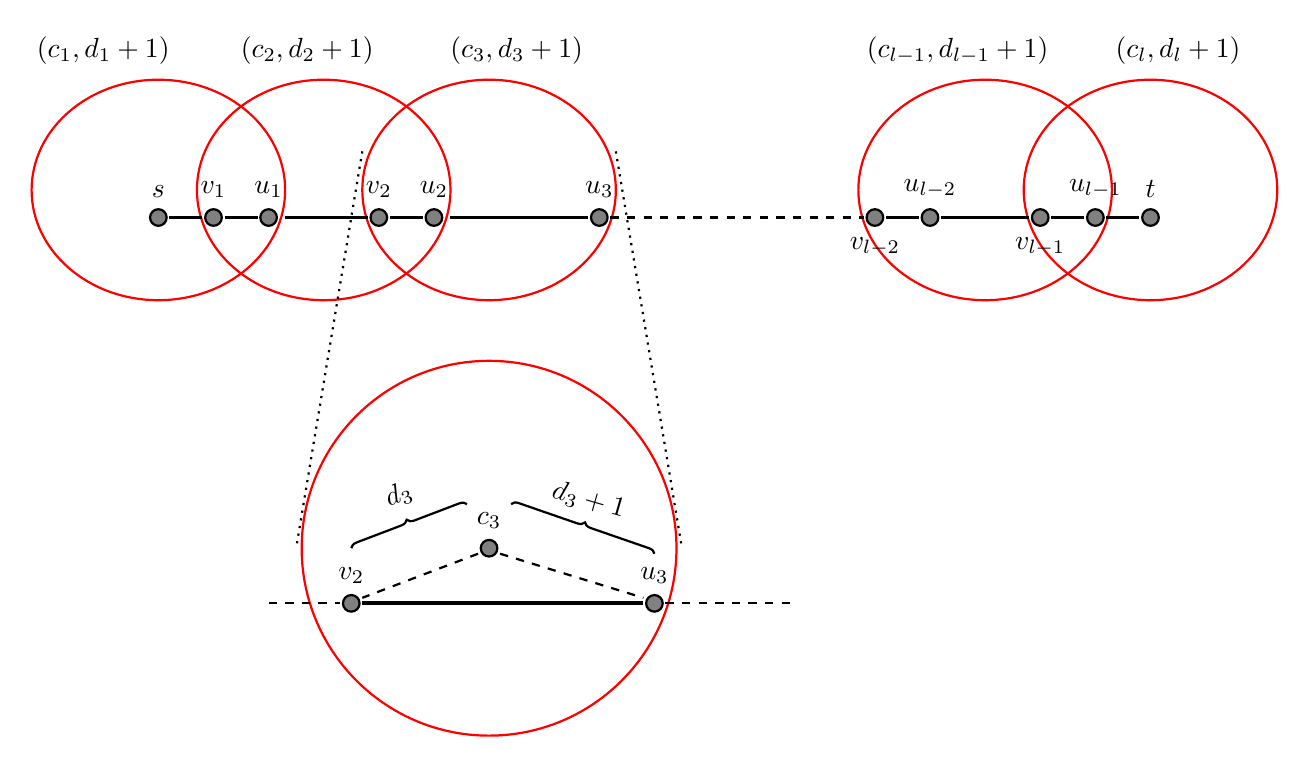
\begin{tikzpicture}[thick,scale=0.7]
	\draw [red] (15, 0.5) ellipse (2.3 and 2);
	\draw [red] (0, 0.5) ellipse (2.3 and 2);
	\draw [red] (3, 0.5) ellipse (2.3 and 2);
	\draw [red] (6, 0.5) ellipse (2.3 and 2);
	\draw [red] (18, 0.5) ellipse (2.3 and 2);
	
	\draw (0, 0) node[circle, draw, fill=black!50, inner sep=0pt, minimum width=6pt, label = $s$] {};
	\draw (18, 0) node[circle, draw, fill=black!50, inner sep=0pt, minimum width=6pt,label = $t$] {};
	
	\draw (2, 0) node[circle, draw, fill=black!50, inner sep=0pt, minimum width=6pt,label = $u_1$] {};
	\draw (1, 0) node[circle, draw, fill=black!50, inner sep=0pt, minimum width=6pt,label = $v_1$] {};
	\draw [line width = 0.5mm] (0.2, 0) -- (0.8, 0);
	\draw [line width = 0.5mm] (1.2, 0) -- (1.8, 0);
	
	\draw (-1, 2.4) node[red, label={$\ball(c_1, d_{1}+1)$}]{};
	
	\draw (5, 0) node[circle, draw, fill=black!50, inner sep=0pt, minimum width=6pt,label = $u_2$] {};
	\draw [line width = 0.5mm] (2.3, 0) -- (3.8, 0);
	\draw [line width = 0.5mm] (4.2, 0) -- (4.8, 0);
	
	\draw (2.7, 2.4) node[red, label={$\ball(c_2, d_{2}+1)$}]{};
	
	\draw (4, 0) node[circle, draw, fill=black!50, inner sep=0pt, minimum width=6pt,label = $v_2$] {};
	\draw (8, 0) node[circle, draw, fill=black!50, inner sep=0pt, minimum width=6pt,label = $u_3$] {};
	\draw [line width = 0.5mm] (5.3, 0) -- (7.8, 0);
	
	\draw (6.5, 2.4) node[red, label={$\ball(c_3, d_{3}+1)$}]{};
	
	\draw[dotted] (3.7, 1.2) -- (2.5, -6);
	\draw[dotted] (8.3, 1.2) -- (9.5, -6);
	\draw (3.5, -7) node[circle, draw, fill=black!50, inner sep=0pt, minimum width=6pt,label = $v_2$] {};
	\draw (9, -7) node[circle, draw, fill=black!50, inner sep=0pt, minimum width=6pt,label = $u_3$] {};
	\draw (6, -6) node[circle, draw, fill=black!50, inner sep=0pt, minimum width=6pt,label = $c_3$] {};
	\draw [red] (6, -6) ellipse (3.4 and 3.4);
	\draw [line width = 0.5mm] (3.7, -7) -- (8.8, -7);
	\draw [dashed] (2, -7) -- (3.3, -7);
	\draw [dashed] (9.2, -7) -- (11.5, -7);
		\draw [decorate,
	decoration = {brace}] (3.5,-6) -- (5.6,-5.2);
	\draw (4.5, -5.6) node[label={[rotate=20]$d_3$}]{};
	\draw [dashed] (5.8, -6.1) -- (3.7, -6.9);
	\draw [decorate,
	decoration = {brace}] (6.4,-5.2) -- (9,-6.1);
	\draw (7.7, -5.7) node[label={[rotate=-16]$d_3+1$}]{};
	\draw [dashed] (6.2, -6.1) -- (8.8, -6.9);
	
	\draw (16, 0) node[circle, draw, fill=black!50, inner sep=0pt, minimum width=6pt,label = -90: $v_{l-1}$] {};
	\draw (17, 0) node[circle, draw, fill=black!50, inner sep=0pt, minimum width=6pt,label = $u_{l-1}$] {};
	\draw [line width = 0.5mm] (17.8, 0) -- (17.2, 0);
	\draw [line width = 0.5mm] (16.8, 0) -- (16.2, 0);

	
	\draw (18.5, 2.4) node[red, label={$\ball(c_l, d_{l}+1)$}]{};
	
	\draw (13, 0) node[circle, draw, fill=black!50, inner sep=0pt, minimum width=6pt,label = -90 : $v_{l-2}$] {};
	\draw (14, 0) node[circle, draw, fill=black!50, inner sep=0pt, minimum width=6pt,label = $u_{l-2}$] {};
	\draw [line width = 0.5mm] (13.8, 0) -- (13.2, 0);
	\draw [line width = 0.5mm] (15.8, 0) -- (14.2, 0);
	
	\draw (14.5, 2.4) node[red, label={$\ball(c_{l-1}, d_{{l-1}}+1)$}]{};
	
	\draw [dashed] (8.2, 0) -- (12.8, 0);
\end{tikzpicture}
	\end{center}
	\caption{The construction of sequences $u_1, u_2, \ldots, u_l$ and $v_1, v_2, \ldots, v_{l-1}$.}\label{terminal}
\end{figure}
%
%Pick the shortest path $\pi$ from $s$ to $t$ under the random perturbations. During the iterations, we will maintain two sequences of vertices $u_0 = s, u_1, u_2, \cdots, u_l$, $v_0 = s, v_1, v_2, \cdots, v_{l-1}$, a sequence of paths $\beta_1, \beta_2, \cdots, \beta_l$, and a sequence of small balls $\ball(c_1, r_{1}), \ball(c_2, r_{2}), \cdots, \ball(c_l, r_{l})\in \clusters$, with the following properties.
\iffalse
\begin{enumerate}[(i)]
\item %$u_1, u_2, \cdots, u_l$, $v_1, v_2, \cdots, v_{l-1}$ are vertices on $\pi$ following the direction from $s$ to $t$, 
for each $1\leq i\leq l-1$, $v_i$ on the sub-path $\pi[u_{i-1}, u_i], \forall 1\leq i\leq l-1$.
\item $v_0\in \ball(c_1, d_{1})$, and $v_i\in \ball^=(c_{i+1}, d_{{i+1}}), u_i\in \ball^=(c_i, d_{i}+1), \forall 1\leq i\leq l-1$. Also, if $u_l\neq t$, $u_l\in \ball^=(c_l, d_{l}+1)$.
\end{enumerate}
\fi

This is done via an iterative process described as the following steps. 

\begin{enumerate}[(1),leftmargin=*]
	\item Start with $i=0$ and set $u_0=v_0=s$. If $u_i = t$ then we terminate the process and set $l=i+1$.
	
	Otherwise, we find the ball in $\clusters_1$ that, among all balls in $\clusters_1$ that intersects $\pi[s, u_i]$, the one that contains a vertex on $\pi$ that is \textbf{closest} to $t$. In other words, if we denote $\pi$ as $(s=w_0,w_1,\ldots,w_{k-1},w_k=t)$, then we find the ball that intersects $\pi[s, u_i]$, and, subject to this, contains a vertex $w_j$ with the largest index.
	
	Note that such a ball always exists; for example, we can take an arbitrary ball in $\bset_1$ that contains $u_i$, and we can also notice that $u_{i+1}$ should belong to $\pi(u_i, t]$.
	
	We denote this ball by $\ball(c_{i+1}, d_{i+1})$ and set $u_{i+1}$ as the last vertex of $\pi$ that belongs to  $\ball(c_{i+1}, d_{i+1}+1)$. 
	
	\item If $i\ge 1$, we then let $v_i$ be any vertex that belongs to both $\pi[u_{i-1}, u_i]$ and $\ball^=(c_{i+1}, d_{i+1})$. We will prove shortly that such $v_i$ always exists.
	
	Then, increase $i\leftarrow i+1$ and go to Step (1).
\end{enumerate}

We now turn to argue the existence of $v_i$.

\begin{claim}
For each $i\ge 1$, $\pi[u_{i-1}, u_i]$ intersects with $\ball^=(c_{i+1}, d_{i+1})$, and if $u_{i+1}\neq t$, then $u_{i+1}\in \ball^=(c_{i+1}, d_{i+1}+1)$.
\end{claim}
\begin{proof}[Proof of claim]
First, if $\pi[s, u_i]$ does not intersect $\ball^=(c_{i+1}, d_{i+1})$, as $\pi[s, u_i]$ intersects $\ball(c_{i+1}, d_{i+1})$, it has to lie entirely within $\ball(c_{i+1}, d_{i+1})$, a contradiction to the choice of $\ball(c_1, d_{1})$ and $u_1$. Therefore, $\pi[s, u_i]$ intersect $\ball^=(c_{i+1}, d_{i+1})$. 

We now claim any such intersection $v_i$ must belong to $\pi[u_{i-1}, u_i]$. Otherwise, if $v_i$ belongs to $\pi[u_{j-1}, u_j]$ for some index $1\leq j<i$, then earlier when we were determining $u_{j+1}$, it should have been at least as close to $t$ as $u_{i+1}$, a contradiction to the property that $u_i\in (u_j,t]$.
%\tnote{According to this new definition, it is not guaranteed that $u_i\in (u_j, t]$.}
%

Lastly, if $u_{i+1}\in \ball(c_{i+1}, d_{i+1})$, then the next vertex on path $\pi$ should also belong to $\ball(c_{i+1}, d_{i+1}+1)$, a contradiction to the choice of $u_{i+1}$.
\end{proof}
		
%Finally, assign $\ball(c_{l+1}, d_{{l+1}})\leftarrow \ball(c, r)$, and increment $l\leftarrow l+1$ and go to Step (2).
%\end{enumerate}
	
It is clear that when the iterative process terminates, $u_l = t$. We now show that for each $2\leq i\leq l-1$, the subpath $\pi[v_{i-1}, u_i]$ is contained in $H$. Note that $v_{i-1}\in \ball^=(c_i, d_{i})$ and $u_i\in \ball^=(c_i, d_{i}+1)$. Since $\ball(c_i, r_{i})$ is small, from the algorithm, we have constructed a subgraph $L_c$ in $G[\ball(c_i, 4r_{i})]$ that preserves all-pairs distances between vertices in $\ball^=(c_i, d_{i})\cup \ball^=(c_i, d_{i}+1)$. As the shortest path between every pair of vertices is unique, the subpath $\pi[v_{i-1}, u_i]$ should be entirely contained in $L_c$.
%\tnote{Shortest paths in unweighted graphs are not unique.}
%by directly adding the shortest paths under random perturbations. Since $\pi$ is the shortest path from $s$ to $t$ under the random perturbations, its sub-path $\pi[v_{i-1}, u_i]$ should belong to the distance preserver which is in spanner $H$. See Figure \ref{terminal} for an illustration.
	
	
Lastly, we consider the distance in $H$ between the endpoints $s, t$ of $\pi$. From the construction, we know that vertices $s, u_1\in \ball(c_1, d_{1}+1)$, and $v_{l-1}, t\in \ball(c_l, d_{l}+1)$. Therefore, $\dist_H(s, u_1) \le  4Rn^\epsilon$, and $\dist_H(v_{l-1}, t) \le 4Rn^\epsilon$. It follows that $\dist_H(s, t)\leq \dist_{G}(s, t) + 8Rn^\epsilon$. Furthermore, if both $s, t$ are covered at boundary by $\clusters_1$, then $s\in \ball^=(c_1, d_{1})$ and $t\in \ball^=(c_l, d_{l})$. Therefore, the entire path $\pi$ belongs to $H$, and so $\dist_H(s, t) = \dist_{G}(s, t)$.
\end{proof}

We now focus on the algorithm for handling large balls.  Consider an iteration in which a shortest path $\pi_{s, t}$ is processed for some pair $s, t\in U$. We prove the following claims.

\begin{claim}\label{boundary}
Let $\pi_{s, t}[u, v]$ be a maximal subpath of $\pi_{s, t}$ consisting of only vertices covered by $\bset_1$. If $u\ne s$ and $v\ne t$, then both $u, v$ are covered at boundary by $\bset_1$.
\end{claim}
\begin{proof}
Assume for contradiction that $u$ belongs to a ball $\ball(c, d-1)$ for some small ball $\ball(c, r)\in\clusters$. Let $(w, u)$ be the last edge of subpath $\pi_{s, t}[s, u]$, then $w\in\ball(c, d)$, and so $w$ is also covered. Therefore, $\pi_{s, t}[w, v]$ should be a covered subpath, which contradicts the maximality of subpath $\pi_{s, t}[u, v]$.
\end{proof}

\begin{claim}\label{Uc}
For any large ball $\ball(c, r)$ and every vertex $s\in U_c$, $\dist_H(s, c)\leq \dist_{G}(s, c) + 10Rn^\epsilon$.
\end{claim}
\begin{proof}
Let $\pi_{s, t}$ be the shortest path that was processed in the iteration where $s$ was added to $U_c$. 
%From the algorithm, we can see that the union of paths in all $\Delta\paths_c$ is equal to the union of all uncovered sub-paths of $\pi_{s, t}$. Therefore, after Step (5), all uncovered sub-paths of $\pi_{s, t}$ are added to spanner $H$. Take an arbitrary sub-path $\pi_{s, t}[u, \cdot]\in \Delta\paths_c$. 
By the algorithm, $\ball(c, r)$ must be referring to some ball $\ball(c_x, r_x)$ for some $x\in \pi_{s, t}$. As $H$ contains a BFS tree that is rooted at $c$ and contains $x$, and the radius of each ball is at most $2Rn^{\eps}$, it suffices to show that $\dist_H(s, x)\leq \dist_{G}(s, x) + 8Rn^\epsilon$.

%Consider all the Type (A) and Type (B) sub-paths on $\pi_{s, t}[s, u]$. Since all Type (B) sub-path edges are now in $H$, we only need to focus on the additive error contributed by Type (A) sub-paths. 
Recall that path $\pi_{s, t}$ was partitioned into subpaths in sets $\Sigma$ and $\Sigma^\prime$. From the algorithm description, all subpaths in $\Sigma'$ are entirely contained in $H$.
For every subpath $\pi_{s, t}[y, z]$ of $\pi_{s, t}$ in $\Sigma$, if $y\neq s$, then from \Cref{exact} and \Cref{boundary}, $\dist_H(y, z) = \dist_{G}(y, z)$; if $y = s$, then from \Cref{exact}, we get that $\dist_H(y, z) \leq \dist_{G}(y, z) + 8Rn^\epsilon$. Since there is at most one subpath $\pi_{s, t}[y, z]$ in $\Sigma$ with $y = s$, the overall additive error caused by subpaths in $\Sigma$ is at most $8Rn^\epsilon$.
\end{proof}

\begin{claim}[additive error]
For every pair  $s, t\in U$, $\dist_H(s, t)\leq \dist_{G}(s, t) + 24Rn^\epsilon$.
\end{claim}
\begin{proof}
Consider the iteration when $\pi_{s, t}$ was processed.
If $\pi_{s, t}$ is entirely covered by $\clusters_1$, %(namely, $\pi_{s, t}$ itself is of Type (A)), 
then the claim follows from \Cref{exact}. 
If not, then from the algorithm, after this iteration some large ball $\ball(c, r)\in\clusters$ intersecting $\pi_{s, t}$ must have added $s, t$ into its set $U_c$. Then from \Cref{Uc}, 
$$\dist_{H}(s, c)\leq \dist_{G}(s, c) + 10Rn^\epsilon,$$
$$\dist_H(c, t)\leq \dist_{G}(c, t) + 10Rn^\epsilon.$$
Let $v$ be an arbitrary vertex in $\ball(c, r)\cap V(\pi_{s, t})$. By triangle inequality,
\[\dist_{G}(s, c) + \dist_{G}(c, t) \leq \dist_G(s, v) + \dist_G(v, t) + 2\cdot \dist(v, c) \leq \dist_G(s, t) + 4Rn^\epsilon.\]
Altogether, $\dist_H(s, t)\leq \dist_{G}(s, t) + 24Rn^\epsilon$.
\end{proof}


\subsection{Size and runtime analysis}

\begin{claim}[spanner size]
$|E(H)|=O\brac{2^{O(1/\epsilon)}\cdot n\log n}$.
\end{claim}
\begin{proof}
\iffalse
From the algorithm, for each large ball $\ball(c,r)\in \bset$, every time a new path is added to $\Pi_c$, the size of $|U_c|$ also increases by at least one, so eventually $|\paths_c|\le |U_c|\le |U|$. As the shortest paths after edge pertubation are unique (and therefore consistent), from \Cref{consist}, 
$$|E(\Pi_c)|\le O(|\ball(c, 4r)| + \sqrt{|\ball(c, 4r)|}\cdot |\paths_c|) \leq O(|\ball(c, 4r)| + \sqrt{|\ball(c, 4r)|}\cdot |U|)\leq O(2^{5/\epsilon}|\ball(c, 4r)|)$$
Summing over all large balls,  $\sum_c|E(\Pi_c)| =\sum_{c}O(2^{5/\epsilon}|\ball(c, 4r)|) = O(2^{15/\epsilon}n/\eps)$. Combined with previous bounds on the number of edges in small balls and in BFS trees, $|E(H)|=2^{O(1/\epsilon)}\cdot n$.
\fi
It suffices to bound the total number of edges added to $H$ when handling large balls. For each large ball $\ball(c, r)\in \bset$, let us conceptually construct a set $\Pi_c$ of paths within $G[\ball(c, 4r)]$ during handling large balls.

Initially, all sets $\Pi_c$ are empty. When processing a path $\pi_{s, t}\in \Pi$, suppose Step (3) is executed. Consider the set of large balls $\{\ball(c_x, r_x)\mid x\in \pi_{s, t} \}$. For any ball $\ball(c, r)\in \{\ball(c_x, r_x)\mid x\in \pi_{s, t} \}$, let $y, z\in \ball(c, r+1)\cap \pi_{s, t}$ be the first and the last vertex on $\pi_{s, t}$. Then, add the subpath $\pi_{s, t}[y, z]$ to $\Pi_c$. Note that this path $\pi_{s,t}$ lies entirely in $G[\ball(c, 4r)]$.

We first show that in the end, all edges added to $H$ for handling large balls is a subset of $E\left(\bigcup_{\ball(c, r)\in \bset\text{ is large}} \Pi_c\right)$. When processing a path $\pi_{s, t}\in \Pi$, consider any vertex $x$ on a sub-path $\rho\in\Sigma^\prime$ which is not an endpoint of $\rho$. Then, since $x$ is not covered by $\bset_1$, any ball that covers $x$ must be large, and in particular $\ball(c_x, r_x)$ should be large. Suppose $y, z\in \ball(c_x, r_x+1)$ are the first and the last vertex on $\pi_{s, t}$. Then, $\pi_{s, t}[y, z]$ must contain all edges incident on $x$ on $\rho$. Hence, the union of all $\pi_{s, t}[y, z]$ ranging over all $x$'s should contain all paths in $\Sigma^\prime$.

Next, we show that $|\Pi_c|\leq |U|$ for any $c$. In fact, each time we added a new path to $\Pi_c$, we must have added $s, t$ to $U_c$ which increased $|U_c|$. Since $U_c\subseteq U$, we know that $|\Pi_c|\leq |U|$ in the end.

Finally, it suffices to bound the number of edges in $E\left(\bigcup_{\ball(c, r)\in \bset\text{ is large}} \Pi_c\right)$. Using \Cref{consist}, we have: 
$$E(\Pi_c)\leq O\left(|\ball(c, 4r)| + \sqrt{\ball(c, 4r)}\cdot |\Pi_c|\right)\leq O\left(|\ball(c, 4r)|\right).$$
Hence, $$E\left(\bigcup_{\ball(c, r)\in \bset\text{ is large}} \Pi_c\right)\leq O\left(\sum_{\ball(c, r)\in \bset\text{ is large}}|\ball(c, 4r)|\right) = O\brac{2^{O(1/\epsilon)}\cdot n\log n}.$$
\end{proof}

\begin{claim}[runtime]
The runtime of the algorithm is $O\big(m\big(|U| + 2^{O(1/\epsilon)}\big)\big)$.
\end{claim}
\begin{proof}
From \Cref{clustering}, computing all the balls in $\clusters$ takes time at most $O(2^{10/\epsilon}m/\eps)$. From \Cref{cor: BFS consistent}, constructing graphs $L_c$ in all small balls takes time at most $O(|U|^{1/2}\sum_c \vol_{G}(\ball(c, 4r)))=O(|U|^{1/2}m \cdot 2^{10/\eps}/\eps)$, and computing the paths in $\Pi$ takes time $O(m|U|)$. As for the part with large balls, the runtime is dominated by scanning all shortest paths $\pi_{s, t}$ in $\Pi$, which takes time at most $O(n|U|)$. Overall, the runtime is $O\big(m\big(|U| + 2^{O(1/\epsilon)}\big)\big)$.
\end{proof}
